\subsection{Deleting vs. removing elements from diagrams} 

A central feature that new users should understand as soon as possible is the way EA handles diagrams. \emph{A diagram is simply treated as a \emph{view} of the
complete model.} The complete model can always be browsed in its entirety via a tree view in the package browser. This space contains all elements that will be
exported. The driving reason behind this setup is that diagrams typically do not contain all elements and one usually uses multiple (possibly redundant)
diagrams to show the different parts of the model. Thinking in this frame is crucial and provides a pragmatic solution to the problem of having huge,
unmaintainable diagrams.

A tricky consequence one must get used to is that removing an element from a diagram does \emph{not} delete it from the model. We have added some support
with the validation in the eMoflon add-in control panel, which can prompt a warning when an element cannot be found in any diagram,\footnote{Review Part II,
Section 2.8 for an example} but there's currently no way to recover a deleted element.

A common mistake new users make is to remove an element by pressing \texttt{del}, and expecting the element to be deleted from the model. As you can probably
guess, this is not the case as evidenced in the package browser (Fig.~\ref{ea:partiallyDeleted}).

\vspace{0.5cm}

\begin{figure}[htbp]
\begin{center} 
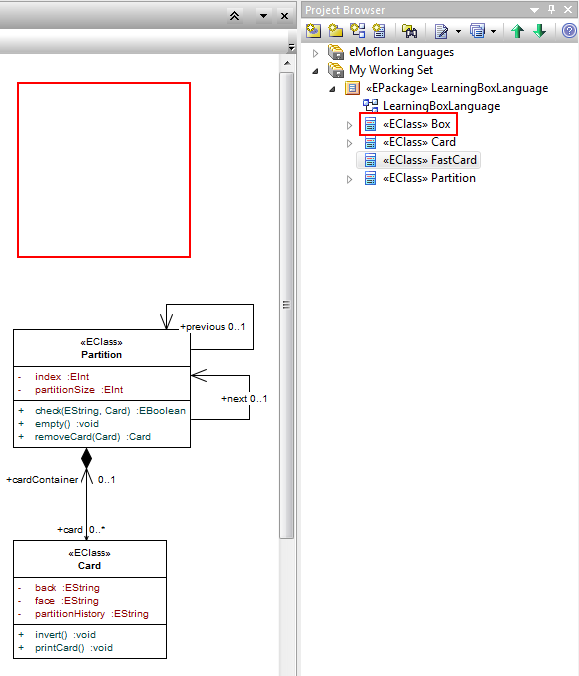
\includegraphics[width=0.6\textwidth]{ea_partiallyDeleted}
  \caption{Removing an element from a diagram via pressing \texttt{Del} does not delete it from the model and it is still present in the package browser}  
    \label{ea:partiallyDeleted}
\end{center}
\end{figure}  

\begin{itemize}
\item[$\blacktriangleright$] To fully delete an element from a model (not just a diagram), select it in the diagram and press \texttt{Ctrl + Del}. Confirm the
action in the warning dialogue (Fig.~\ref{ea:deleteWarning}), and the element should no longer be in the project browser.

\vspace{0.5cm}

\item[$\blacktriangleright$] Alternatively, elements can be deleted directly from project browser by right-clicking the item and navigating to the large
red `x' at the bottom of the context menu

\begin{figure}[htbp]
\begin{center}
  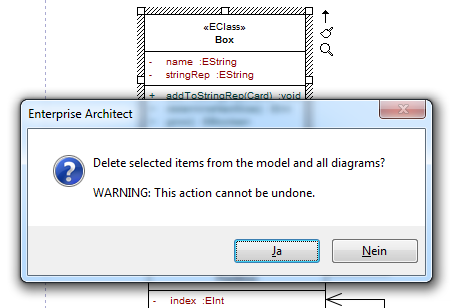
\includegraphics[width=0.7\textwidth]{ea_deleteWarning}
  \caption{Deleting an element from a diagram and the model}  
  \label{ea:deleteWarning}
\end{center}
\end{figure}  

\end{itemize}
